If $L$ has the same complexity of $H$, namely $L \leq_{p} H$, then $H$ is at least as hard as $L$, at least as far as classes like \textbf{P} are concerned. \vspace{7pt}

The previous statement simply says: if $L \leq_{p} H$ and $H \in \textbf{P}$, then also $L \in \textbf{P}$. A possible method to solve $L$ in this case 
is to take an instance of $L$ and translate it into an instance of $H$, namely $f(x)$, which must be done in polynomial time: checking whether $f(x) \in H$ gives 
the answer to the original question, $x \in L$. \vspace{7pt}

Suppose we have a problem $H \subseteq \{0,1\}^*$. It's said to be:
\begin{itemize}
    \renewcommand{\labelitemi}{-}
    \item \textbf{NP}-hard if $L \leq_{p} H$ for every language $L\in \text{NP}$.
    \item \textbf{NP}-complete if $H$ is \textbf{NP}-hard, and $H \in \text{NP}$.
\end{itemize}
More in details, \textbf{NP}-hard defines all the problems that have a difficulty greater than any other language $L$ inside \textbf{NP}. However, 
this does not mean that $H$ is in \textbf{NP}, we are just stating that the problem $H$ is more difficult than any other problem in \textbf{NP}. \vspace{7pt}

In the other hand, \textbf{NP}-complete defines all the problems $H$ already in \textbf{NP} that are more difficult than any other problem in \textbf{NP}.
\begin{definition}[title = Theorem]
    \begin{enumerate}
        \item The relation $\leq_{p}$ is a pre-order (\textit{i.e. it is reflexive and transitive, meaning that any language $L$ is at least as difficult as the language itself and we can form chains of reductions to find out the complexity of a given decision problem}).
        \item If $L$ is \textbf{NP}-hard and $L \in \textbf{P}$, then $\textbf{P} = \textbf{NP}$.
        \item If $L$ is \textbf{NP}-complete, then $L \in \textbf{P}$ if and only if $\textbf{P} = \textbf{NP}$.
    \end{enumerate}
\end{definition}
Let's take a look at the following representation.
\begin{center}
    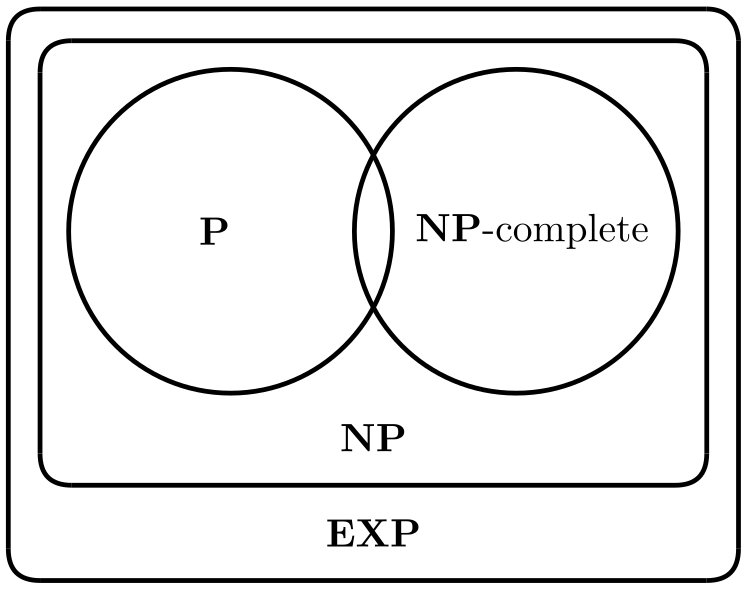
\includegraphics[width = 0.5\textwidth]{img/img6.png}
\end{center}
From the picture above, we get how the complexities are related between each other, in particular:
$$\text{P} \subseteq \text{NP} \subseteq \text{EXP}$$
The intersection between P and NP-complete is an empty area: they are completely disjointed. Therefore, P and NP-complete can be seen as extremes of the 
complexity class NP: P is the easiest extreme while NP-complete is the hardest extreme. 